
\subsection{Simulation method}

This part will analyze the effect of several parameters on 3 aspects of the result, which is the probability of creating barrier, the average exposure along the multiple view barrier coverage and the overall computational time. The algorithm is performed on every instance and keep recording 3 data, the creation of barrier, the computation time and the exposure on a barrier if there is one. Then, the result are combined for all instances of the same parameter settings to achieve the probability of barrier creation, the average computational time and the average exposure value on the found barriers.

\subsection{System setting and parameters setting}
%Đoạn này hư cấu sửa sau :v
System settings

All the experiments are performed on a personal computer with core Intel Core i7-7700HQ, 8GB of DDR4 RAM running on Windows 10 Home, the programming language used to simulate the algorithm is Java 11.

Parameter settings

The sensing fields in all experiments are presented as rectangles with the size of 200m x 50m. Sensor nodes are deployed uniformly randomly in a rectangle with each side extended compared to the sides of the sensing field a distance equal to the sensing radius of each sensor in order to guarantee the uniform distribution regarding sensing area inside the sensing field. Each set of parameters contains several independent random topologies to conduct the algorithm on and measure the target indexes. Altogether there are 21000 experiments on 210 instances of parameters which were analyzed with our algorithm. The details are as follows:
\begin{table}[h!]
	\centering
	\begin{tabular}{l | r}
		Length & 200 \\
		Width & 50 \\
		Sensing Radius & 30 \\
		Minimum sensing radius & 5 \\
		Sensing angle & 90 \\
		k & 3, 4, 5, 6 \\
		The number of topologies for each instance & 100
	\end{tabular}
	\caption{General parameters}
\end{table}

\begin{table}[h!]
	\centering
	\begin{tabular}{l | c | c | c | c}
		k & 3 & 4 & 5 & 6\\
		$\omega$ & 90 - 115 & 55 - 80 & 40 - 60 & 35 - 50\\
	\end{tabular}
	\caption{Problem parameters}
\end{table}

\subsection{Computation results}

\subsubsection{Effect of $\omega$ on algorithm performance}

$\omega$ is an important parameter in the $k-\omega$ coverage model. As a result, this parameter has a considerable impact on the output of the algorithm. Because $\omega$ is a lower bound for the angle between two consecutive sensors in the perspective of the considered point, every sensor set that satisfies the condition with large $\omega$ would also successfully make a $k-\omega$ cover with lower $\omega$. In short, a decrease in parameter $\omega$ may result in an expansion in the result space of the algorithm. This leads to two different consequences. On the one hand, there would be more sets of sensor $k-\omega$ cover a single node, which means that the exposure of that node is likely to be lifted. However, on the other hand, the lower value of $\omega$ could reduce the average rank of the covered nodes, as the nodes are more easily covered, which leads to a lower exposure, since the sets that cover the bigger node tend to position further than the sets covering the smaller ones.

As a consequence, firstly, with a lower value of $\omega$, the algorithm would offer a greater chance of $(k-\omega)$ barrier existence, and probably also a greater exposure on the obtained barriers. However, the probability of forming barriers can never exceed $100\%$, the curve that represents the barrier probability would approach $100\%$ and does not rise higher with lower $\omega$. Furthermore, a high exposure usually occurs when the node is exposed at every direction, which may satisfy the condition with high $\omega$. Consequently, the exposure value would eventually approach a bound when the value of $\omega$ decrease.

On the other hand, a lower value of $\omega$ results in a larger searching space, which leads to a drastic rise in computation time. As a result, it is suitable to choose a sufficient $\omega$ so that the barrier probability and the barrier exposure approach its upper bound while the computation time is still acceptable.

\begin{figure}[h]
	\begin{subfigure}[t]{.5\textwidth}
		\centering
		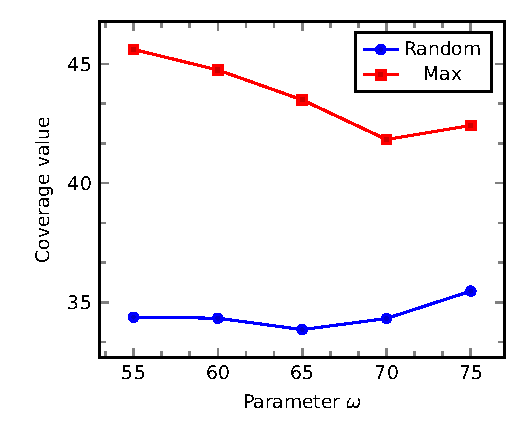
\includegraphics[scale=.8]{Hinhanh/OmegaEffect/coverage/k4.pdf}
		\caption{k = 3}
	\end{subfigure}
%	\hfill
	\begin{subfigure}[t]{.5\textwidth}
		\centering
		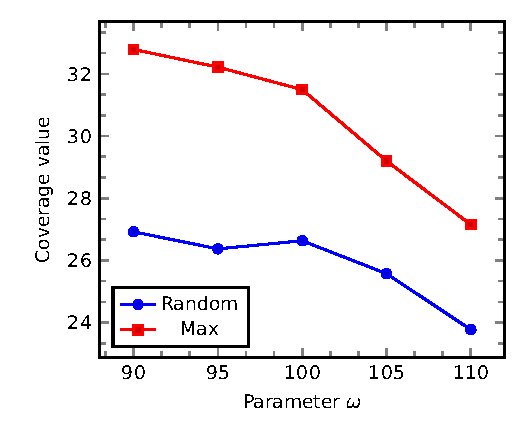
\includegraphics[scale=.8]{Hinhanh/OmegaEffect/coverage/k3.pdf}		
		\caption{k = 4}
	\end{subfigure}
\caption{}
\label{fig:}
\end{figure}
%
\begin{figure}[h]
	\begin{subfigure}[t]{.5\textwidth}
		\centering
		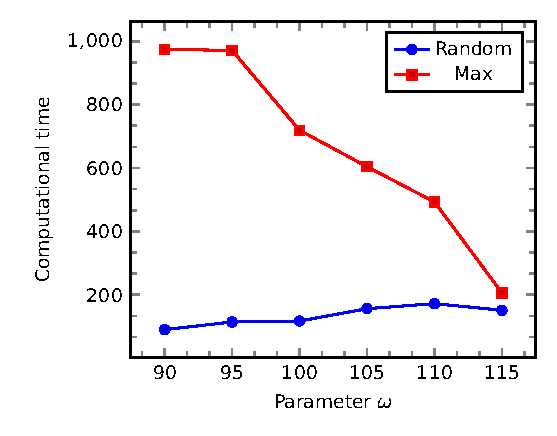
\includegraphics[scale=.8]{Hinhanh/OmegaEffect/time/k3.pdf}		
		\caption{k = 3}
	\end{subfigure}
	\begin{subfigure}[t]{.5\textwidth}
		\centering
		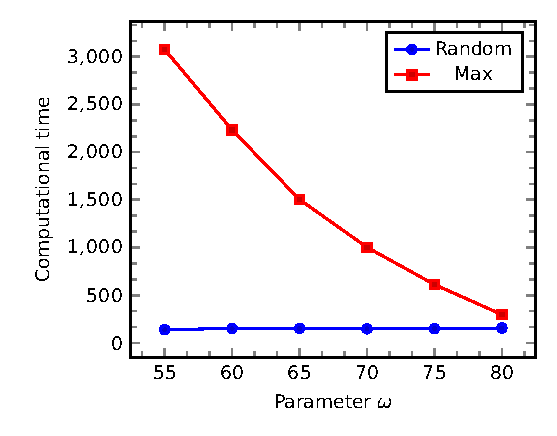
\includegraphics[scale=.8]{Hinhanh/OmegaEffect/time/k4.pdf}		
		\caption{k = 4}
	\end{subfigure}
\caption{}
\label{fig:}
\end{figure}
%
\begin{figure}[h]
	\begin{subfigure}[t]{.5\textwidth}
		\centering
		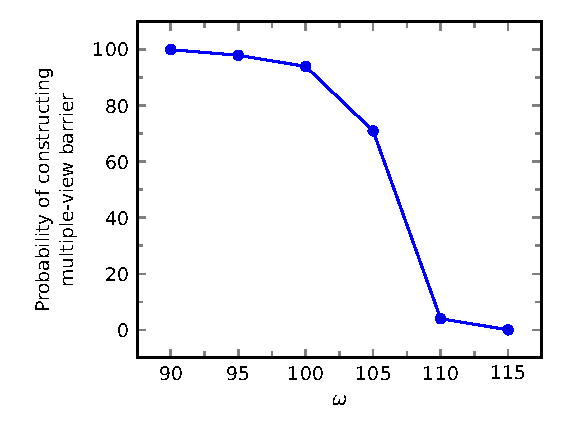
\includegraphics[scale=.8]{Hinhanh/OmegaEffect/probability/k3.pdf}		
		\caption{k = 3}
	\end{subfigure}
	\begin{subfigure}[t]{.5\textwidth}
		\centering
		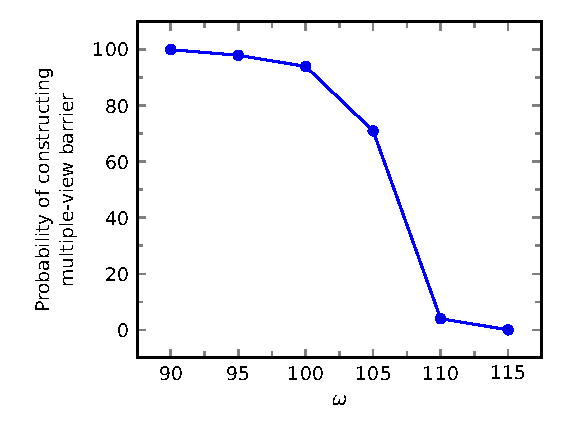
\includegraphics[scale=.8]{Hinhanh/OmegaEffect/probability/k3.pdf}		
		\caption{k = 4}
	\end{subfigure}
\caption{}
\label{fig:}
\end{figure}

\subsubsection{Effect of sensor number on algorithm performance}

Like the effect of $\omega$, a larger value of sensor number would lead to a larger searching space. However, in this occasion, the negative effect on exposure seems to be more important. As a result, the barrier exposure tends to fall slowly as the sensor number rises. Furthermore, the large number of sensors leads to a huge computational work. This results in the computation time surge dramatically as the sensor number grows. Thus, it is suitable to choose a sufficient sensor number so that the barrier probability approaches $100\%$, while the barrier exposure has not fallen too considerable and the computation time is still acceptable.

\begin{figure}[h]
	\begin{subfigure}{.5\textwidth}
		\centering
		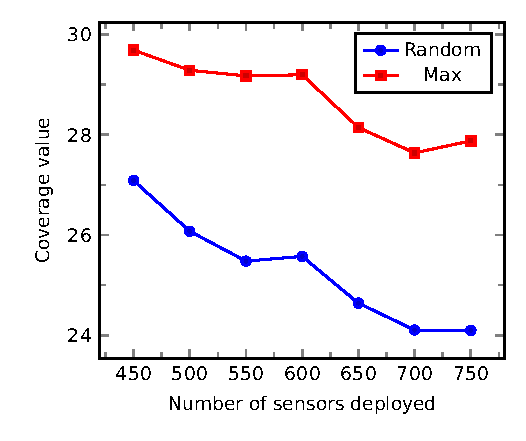
\includegraphics[scale=.8]{Hinhanh/SensorNumberEffect/coverage/k3omega105.pdf}
		\caption{k = 3, $\omega$ = 105}
	\end{subfigure}
	\begin{subfigure}{.5\textwidth}
		\centering
		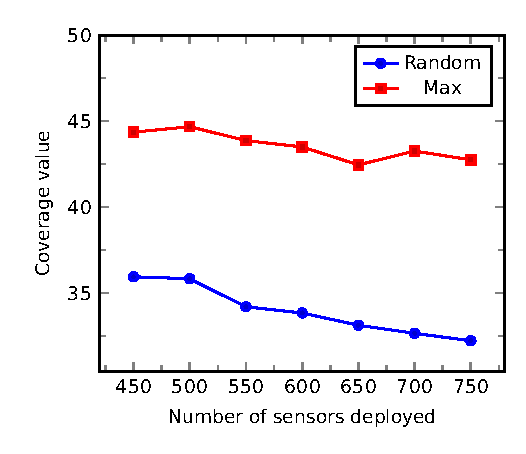
\includegraphics[scale=.8]{Hinhanh/SensorNumberEffect/coverage/k4omega65.pdf}
		\caption{k = 4, $\omega$ = 65}
	\end{subfigure}
\caption{}
\label{fig:}
\end{figure}
%
\begin{figure}[h]
	\begin{subfigure}{.5\textwidth}
		\centering
		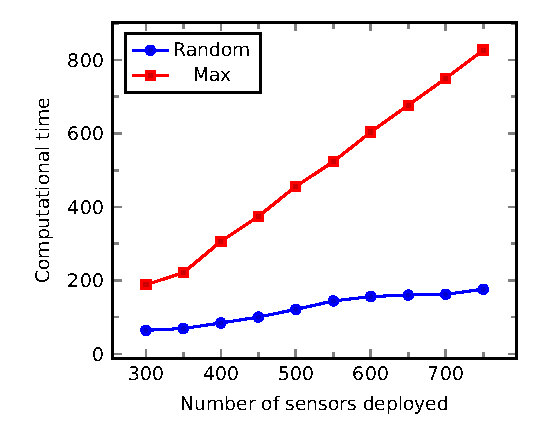
\includegraphics[scale=.8]{Hinhanh/SensorNumberEffect/time/k3omega105.pdf}
		\caption{k = 3, $\omega$ = 105}
	\end{subfigure}
	\begin{subfigure}{.5\textwidth}
		\centering
		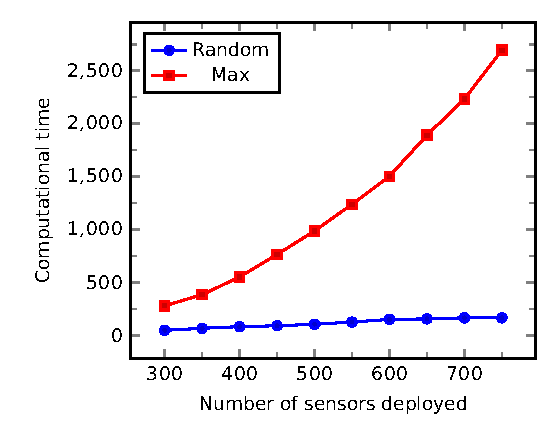
\includegraphics[scale=.8]{Hinhanh/SensorNumberEffect/time/k4omega65.pdf}
		\caption{k = 4, $\omega$ = 65}
	\end{subfigure}
\caption{}
\label{fig:}
\end{figure}
%
\begin{figure}[h]
	\begin{subfigure}{.5\textwidth}
		\centering
		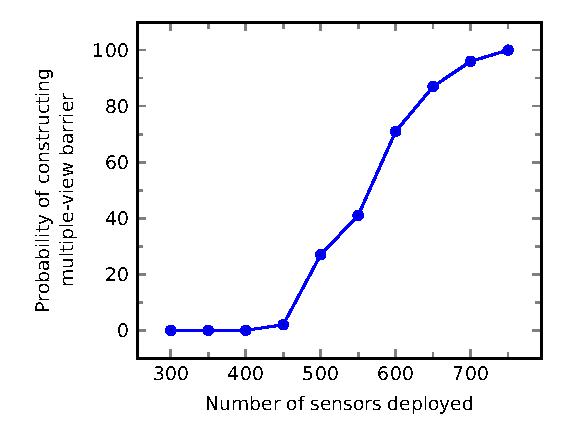
\includegraphics[scale=.8]{Hinhanh/SensorNumberEffect/probability/k3omega105.pdf}
		\caption{k = 3, $\omega$ = 105}
	\end{subfigure}
	\begin{subfigure}{.5\textwidth}
		\centering
		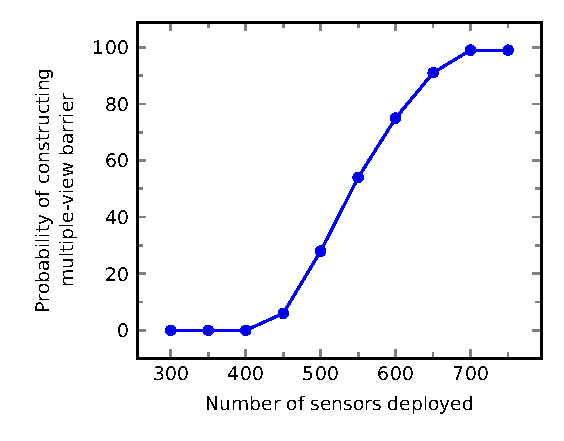
\includegraphics[scale=.8]{Hinhanh/SensorNumberEffect/probability/k4omega65.pdf}
		\caption{k = 4, $\omega$ = 65}
	\end{subfigure}
\caption{}
\label{fig:}
\end{figure}

\subsubsection{Effect of $k$ on algorithm performance}

The parameter$k$ is affected the achieved results the most regarding all 3 aspects. This is because the change in k would manipulate the problem entirely, an answer with a value of $k$ would not be an answer with another value of $k$. As a consequence, the achieved results are drastically different among every value of $k$.

As mentioned in previous parts, generally, the exposure of the barriers would not be much different from the others. As a result, we may reach a conclusion that for every value of $k$, it is possible to define a critical value of barrier exposure which denotes the largest achieved value of exposure for a certain value of $k$. And this critical exposure value could be use to compare the performance of the problem with different values of $k$.

Regarding this metric, in general, as there are more sensors that cover a certain point, an increase in the value of $k$ may lead to a larger critical exposure. However, since the function of $cos(x)$ has a derivative getting lower as the value of $x$ comes close to 0, and the effect of increasing $k$ on decreasing the sight angle of sensors to the parts of the intruder ($\phi - \phi_i$) may reduce with larger $k$. As a result, the critical exposure value will eventually reach a bound when the value of $k$ keep climbing.

Finally, the effect of $k$ on computation time is. This is because that the large value of $k$ would leads to a larger nest in traversing for all the $k-\omega$ sets and larger loop when checking the exposure of nodes, hence the computation time for finding all the sets that $k-\omega$ cover each node and determining the sets of sensor with largest exposure is increased considerably.

In conclusion, there may exist a value of $k$ such that its critical exposure approaches the upper bound while the computation time has not been exceptional.

\begin{figure}[h]
	\centering
	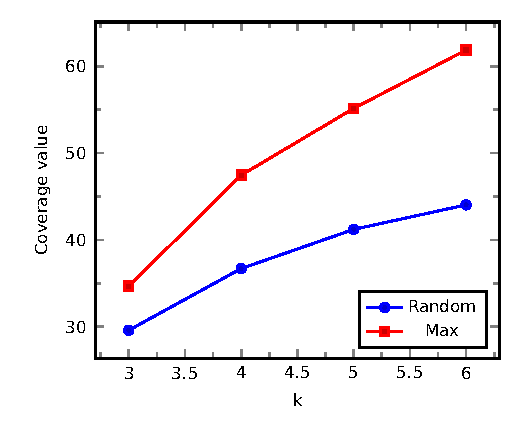
\includegraphics[scale=1.]{Hinhanh/kEffect/main.pdf}
	\caption{}
	\label{fig:}
\end{figure}

\subsubsection{Compare the devised metric with the traditional coverage models}
The figure below illustrates the result of barrier coverage regarding the density computation, which means the coverage of a barrier is calculated as the average of the coverage of every point on the barrier. Practically, the method to evaluate the coverage of a barrier has been proposed in section \ref{baCal}. The assessment takes into consideration 2 attenuated models, which are the Closest-Sensor and the All-Sensor Intensity.

From the above figure, it is obvious that the differential coverage model outperform the tradition ones